\documentclass [t, dvipsnames]{beamer}
\setbeamertemplate{navigation symbols}{}

\usetheme{CambridgeUS}

\usecolortheme{crane}

\useinnertheme{circles}

%%% Работа с русским языком
\usepackage[english,russian]{babel}   %% загружает пакет многоязыковой вёрстки
\usepackage{fontspec}      %% подготавливает загрузку шрифтов Open Type, True Type и др.
\defaultfontfeatures{Ligatures={TeX},Renderer=Basic}  %% свойства шрифтов по умолчанию
\setmainfont[Ligatures={TeX,Historic}]{Times New Roman} %% задаёт основной шрифт документа
\setsansfont{Arial}                    %% задаёт шрифт без засечек
\setmonofont{Courier New}
\usepackage{indentfirst}
\frenchspacing

%%% Дополнительная работа с математикой
\usepackage{amsmath,amsfonts,amssymb,amsthm,mathtools}
\usepackage{icomma} % "Умная" запятая: $0,2$ --- число, $0, 2$ --- перечисление

%% Перенос знаков в формулах (по Львовскому)
\newcommand*{\hm}[1]{#1\nobreak\discretionary{}
	{\hbox{$\mathsurround=0pt #1$}}{}}

%%% Работа с картинками
\usepackage{graphicx}  % Для вставки рисунков
\graphicspath{{images/}{images2/}}  % папки с картинками
\setlength\fboxsep{3pt} % Отступ рамки \fbox{} от рисунка
\setlength\fboxrule{1pt} % Толщина линий рамки \fbox{}
\usepackage{wrapfig} % Обтекание рисунков текстом

%%% Работа с таблицами
\usepackage{array,tabularx,tabulary,booktabs, delarray} % Дополнительная работа с таблицами
\usepackage{longtable}  % Длинные таблицы
\usepackage{multirow} % Слияние строк в таблице
\usepackage{colortbl}

\newcolumntype{Z}[1]{>{\centering\arraybackslash}p{#1cm}}
%%% Программирование
\usepackage{etoolbox} % логические операторы

%%% Другие пакеты
\usepackage{lastpage} % Узнать, сколько всего страниц в документе.
\usepackage{soul} % Модификаторы начертания
\usepackage{csquotes} % Еще инструменты для ссылок
\usepackage{multicol} % Несколько колонок


\usepackage{hyperref}
\usepackage{xcolor}
\hypersetup{        % Гиперссылки
	unicode=true,           % русские буквы в раздела PDF
	pdftitle={Заголовок},   % Заголовок
	pdfauthor={Автор},      % Автор
	pdfsubject={Тема},      % Тема
	pdfcreator={Создатель}, % Создатель
	pdfproducer={Производитель}, % Производитель
	pdfkeywords={keyword1} {key2} {key3}, % Ключевые слова
	colorlinks=true,        % false: ссылки в рамках; true: цветные ссылки
	linkcolor=,          % внутренние ссылки
	citecolor=green,        % на библиографию
	filecolor=magenta,      % на файлы
	urlcolor=blue           % на URL
} 

%%%Заголовки%%
\usepackage{etoolbox}
\setbeamertemplate{headline}
{
	\leavevmode
	\hbox{%
		\begin{beamercolorbox}[wd=.5\paperwidth,ht=2.25ex,dp=1ex,right]{section in head/foot}%
			\usebeamerfont{section in head/foot}\thesection. \insertsectionhead\hspace*{2ex}
		\end{beamercolorbox}
		\begin{beamercolorbox}[wd=.5\paperwidth,ht=2.25ex,dp=1ex,left]{subsection in head/foot}
			\usebeamerfont{subsection in head/foot}
			\ifnumgreater{\arabic{subsection}}{0}{%
			\hspace*{1ex}\thesection.\thesubsection. \insertsubsectionhead}
			{}%
	\end{beamercolorbox}}
	\vskip0pt
}
%%Новое окружение%%
\newenvironment{slide}[1][t]
{\begin{frame}[fragile,environment=slide,#1]
		\frametitle{\thesection. \insertsection}
		\ifnumgreater{\arabic{subsection}}{0}{\framesubtitle{\thesection.\thesubsection. \insertsubsection}}
			{}}
	{\end{frame}}


%%Оглавление перед каждой section%%
\AtBeginSection[]
{
	\begin{frame}[plain]
		\tableofcontents[currentsection]
	\end{frame}
}

\title[Риски на рынке корпоративных облигаций]{Выявление факторов рисков \\
на рынке корпоративных облигаций в России}

\author [Никаноров Иван] {Никаноров Иван Олегович}
\institute [РАНХиГС] {Российская Академия Народного Хозяйства и  \\ Государственной Службы при Президенте Российской Федерации}

\vfill
\date[\today]{\today}

\begin{document}
\frame[plain] {\titlepage}

\frame[plain]{\tableofcontents}

\section{Актуальность}

\begin{slide}
	\begin{itemize}
		\item Облигация является одной из важнейших ценных бумаг. 
		\item Рынок облигаций является самым крупным из рынков ценных бумаг, больше половины оборота которого приходится на корпоративные облигации.
		\item Россия имеет достаточно низкий суверенный рейтинг (BB+ согласно S\&P).
		\item Поскольку рейтинг компании не может быть выше странового рейтинга, в которой эта компания зарегистрирована, низкий страновой рейтинг занижает рейтинги российских эмитентов.
	\end{itemize}
\end{slide}

\section{Цели и задачи исследования}

\begin{slide}
		\textbf{Цель исследования:}\\
		 Анализ факторов рисков на рынке корпоративных облигаций в России
		\vfill
		\textbf{Задачи исследования:}
	\begin{itemize}
		\item Обзор литературы
		\item Сбор и анализ данных
		\item Характеристика рисков, связанных с российскими корпоративными облигациями
		\item Выявление факторов, вызывающих риски, связанные с корпоративными облигациями российских компаний.
		\item Предоставление практических рекомендаций по снижению этих рисков.
	\end{itemize}
\end{slide}

\section{Классификация облигаций}

\begin{slide}[c]
 \centering 	
 \scalebox{0.65}{
 		\begin{tabular}{p{5cm}Z{4}p{7cm}}
 		\hline
 		\multicolumn{1}{Z{5}}{Классификационный признак} & Влияние на оценку стоимости & \multicolumn{1}{Z{7}}{Виды облигаций} \\ 
 		\hline
 		\only<2->{Эмитент & Нет   & Государственные, муниципальные, корпоративные \\
 		\hline}
 		\only<3-> {По площадке размещения & Нет   & Еврооблигации (евробонды), иностранные, международные, глобальные \\
 		\hline}
 		\only<4->{Легитимации владения & Нет   & Именные, на предъявителя, с отрывным купоном \\
 		\hline}
 		\only<5->{Обеспеченность & Нет   & Необеспеченные, обеспеченные \\
 		\hline}
 		\only<6->{Срок погашения & Да    & Краткосрочные, среднесрочные, долгосрочные, бессрочные \\
 		\hline}
 		\only<7->{Возможность продления срока & Да    & Непродлеваемые, продлеваемые (пролонгируемые) \\
 		\hline}
 		\only<8->{Возможность досрочного погашения & Да    & Безотзывные, отзывные \\
 		\hline}
 		\only<9->{Погашение номинала & Да    &  Одним платежом в конце срока, амортизируемые, смешанные \\
 		\hline}
 		\only<10->{Формирование дохода & Да    & С фиксированным купоном, с плавающим купоном, индексируемые \\
 		\hline}
 		\only<11->{Способ выплаты дохода & Да    & Процентные, бескупонные \\
 		\hline}
 		\only<12->{Обращение & Да    & Конвертируемые, неконвертируемые \\
 		\hline}
 	\end{tabular}%
 }
\end{slide}

\section{Эмпирика}
\subsection{Собранные данные}

\begin{slide}
	\alt <2> {Из этих двух создан список эмитентов, входящих в РБК-500, с указанием количества выпусков у каждого эмитента. Всего 45 эмитентов и 340 выпусков.}{
 \begin{enumerate}
 	\item Данные о 469 облигациях, номинированных в рублях, с сайта Cbonds, эмитенты которых имеют рейтинг агентства S\&P в нац. валюте (рублях) с указанием отрасли, к которой относится эмитент
 	\item Список 500 компаний, входящих в рейтинг РБК-500 с указанием отрасли
 \end{enumerate}}
\end{slide}

\subsection{Распределение кредитных рейтингов по отраслям}

\begin{slide}[t]
 \alt<3> {И в итоге было получено следующее:}{Сначала было посчитано число эмитентов в каждой отрасли и получено вот это:} %Да, это левый порядок, но почему-то по-русски он работать не хочет :((
 \temporal<2>{
 	\begin{center}
 		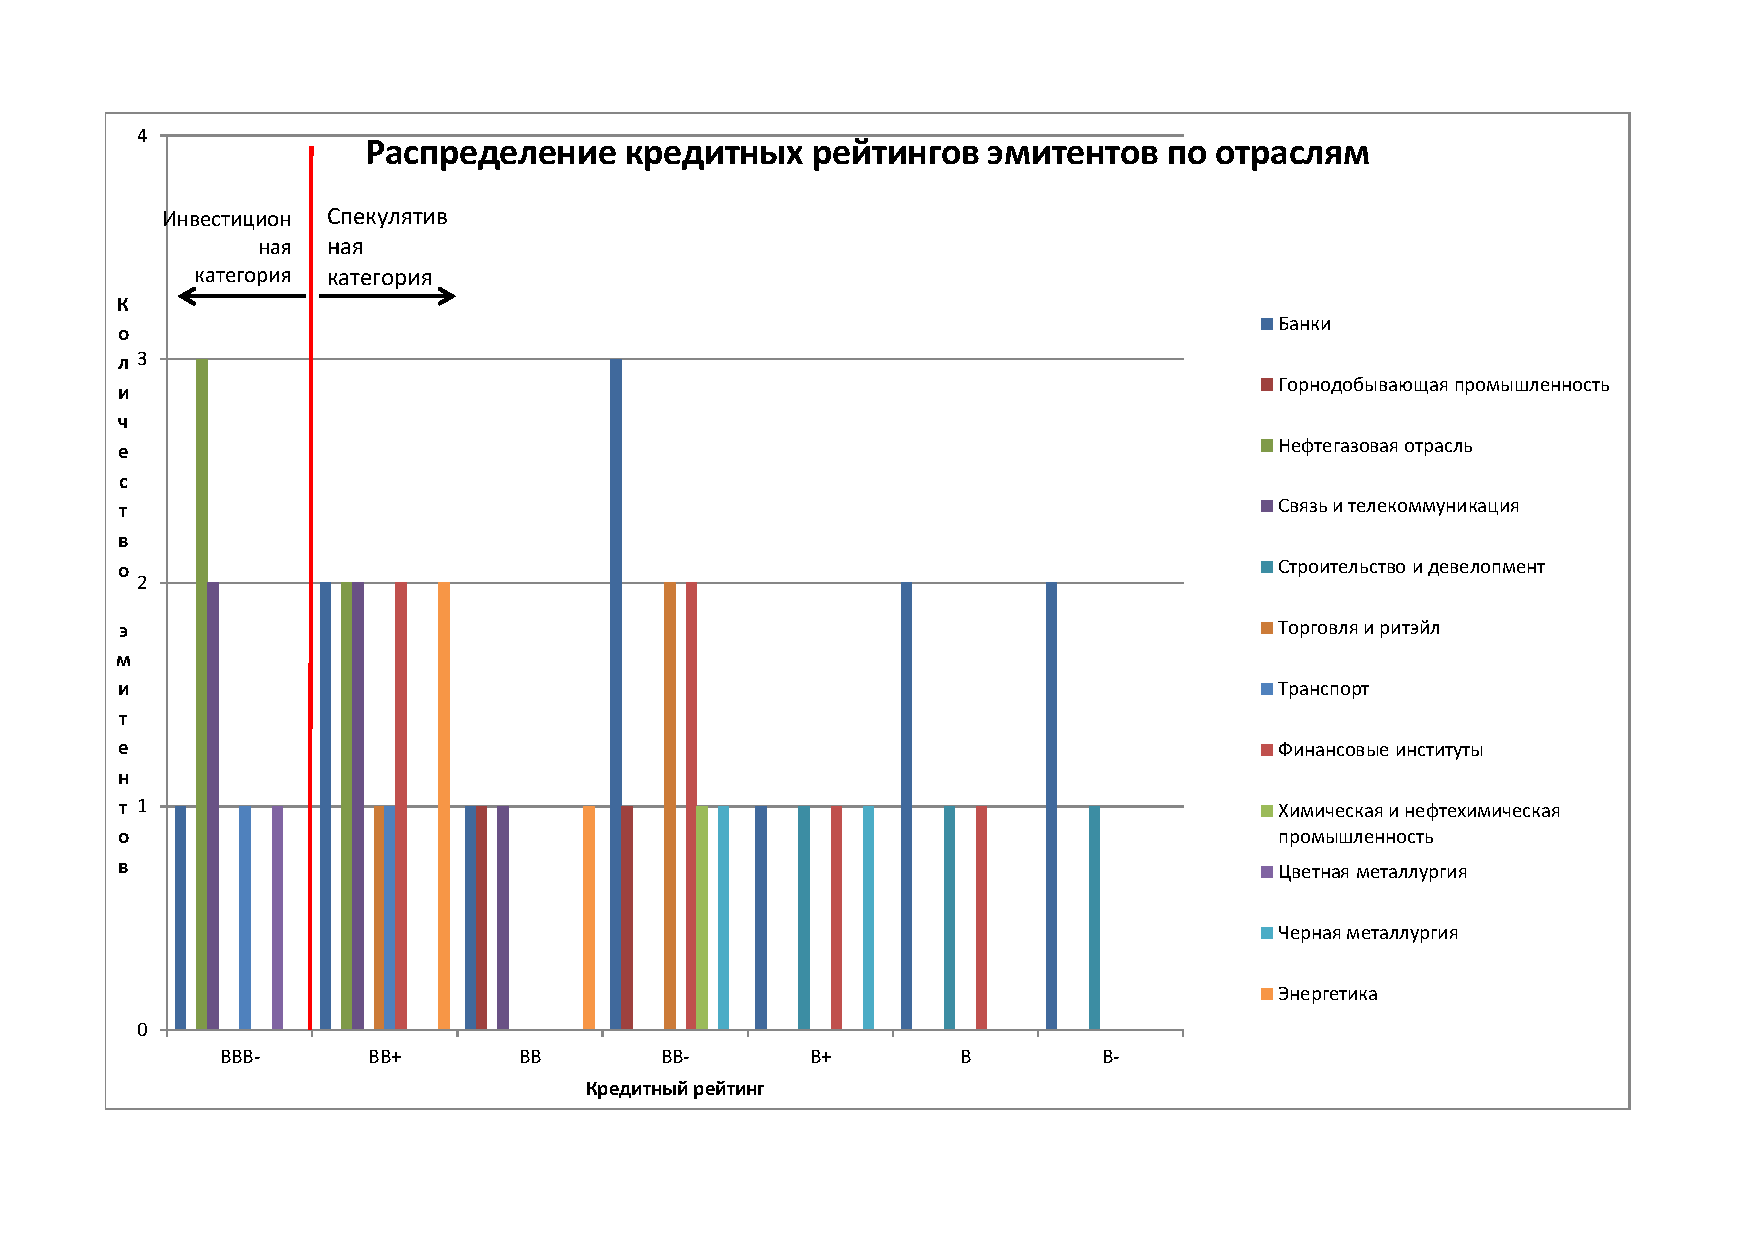
\includegraphics[height=6.8cm, width=12cm, trim= 1.8cm 0 1cm 19.2mm, clip]{Credit_ranks_01.pdf}
 	\end{center}} {
	\\
	\vspace{2.5cm}
 	Затем было учтено количество выпусков каждого эмитента}{
 	\begin{center}
 		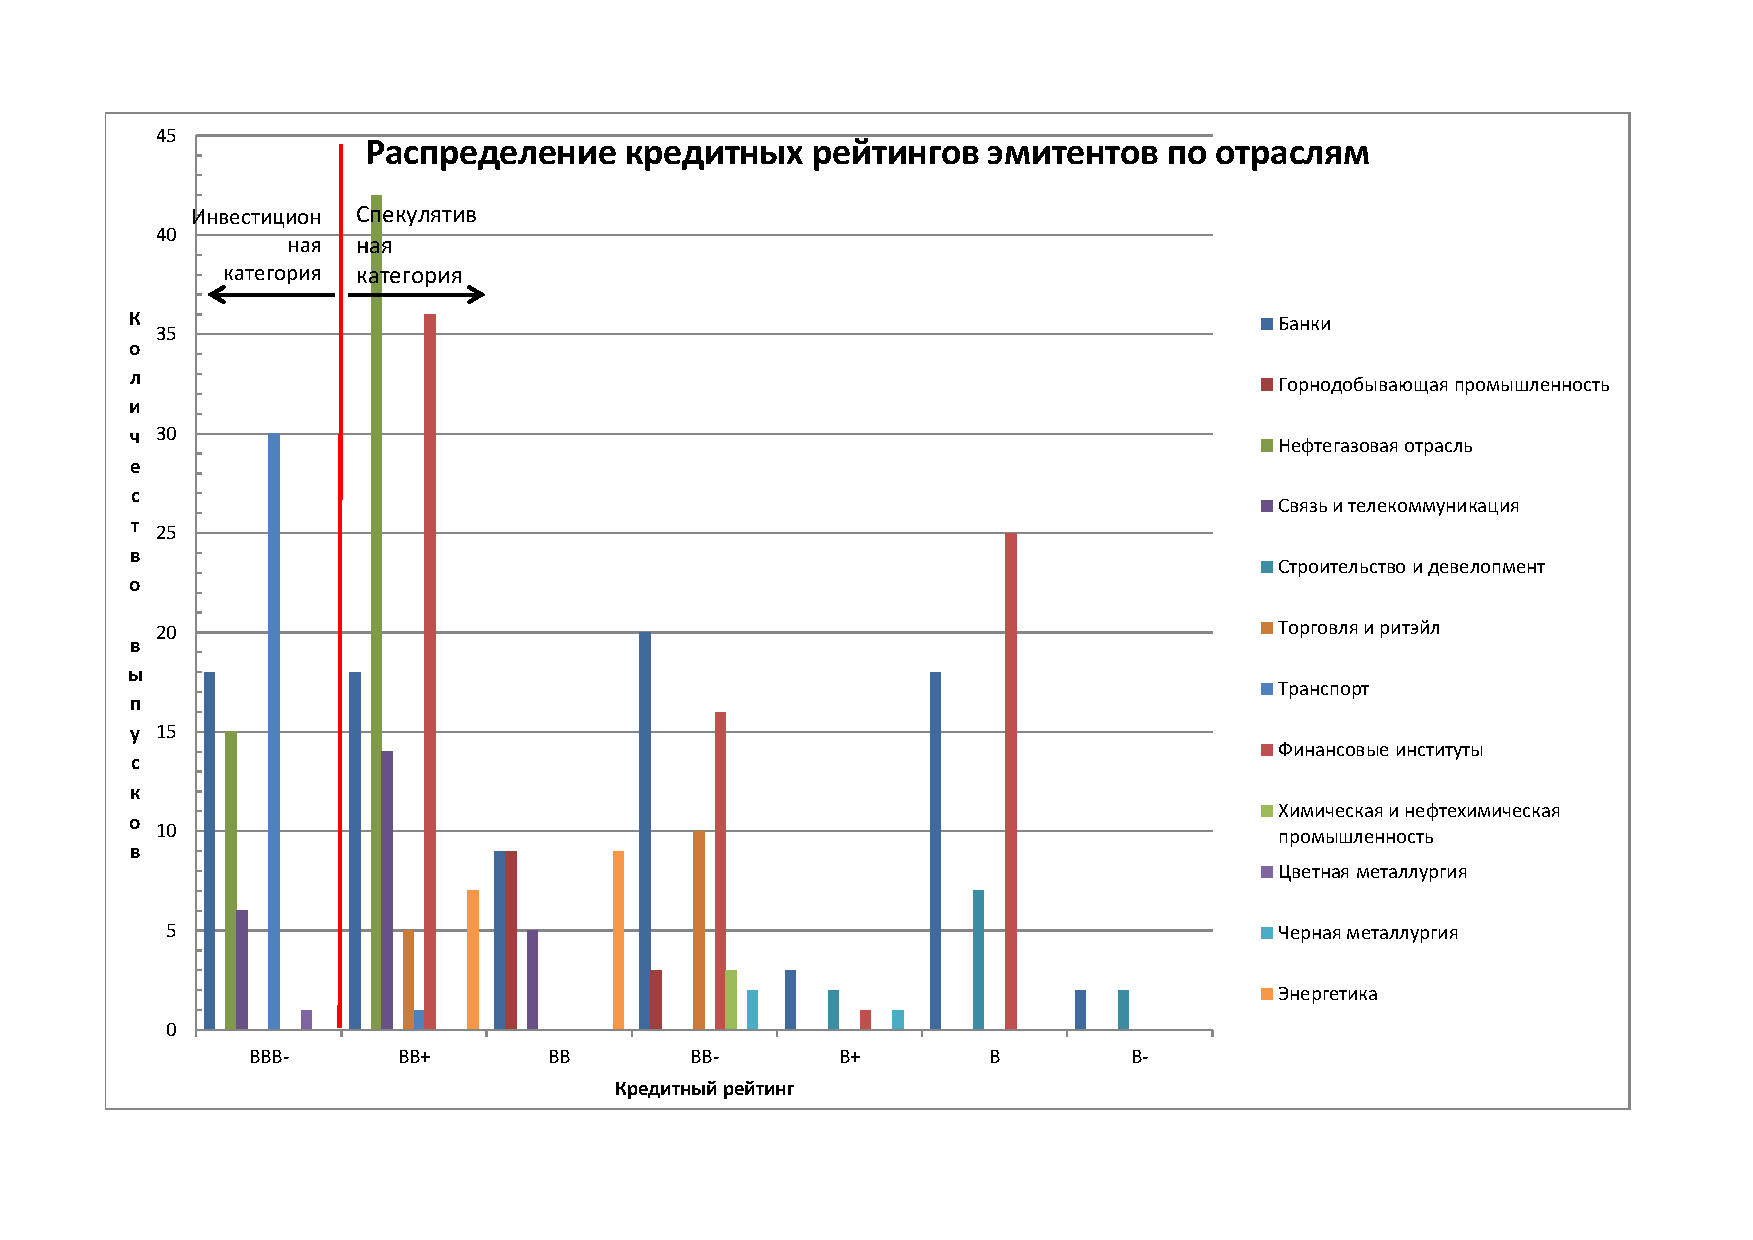
\includegraphics[height=7.3cm, width=12cm, trim= 1.8cm 0 1cm 19.4mm, clip]{Credit_ranks_02.pdf}
	 \end{center}}
\end{slide}

\frame[plain, c] {\centering
	Спасибо за внимание!}

\end{document}